\section{Digitālas aparatūras projektēšana}

Lai digitalizētu \glslink{firmware}{programmaparatūras} jeb digitālu iekārtu
prototipēšanas fāzi, ir nepieciešams saprast, ko nozīmē prototipēt jeb
izstrādāt, jeb projektēt digitālu aparatūru.  
  
Digitālās aparatūras projektēšana sevī ietver 1) signālus, 2) loģiskus
elementus, 3) vadus starp tiem loģiskajiem elementiem, 4) šo elementu
izvietošanu integrētā shēmā. 
  
Vērtīgi pieminēt, ka loģiskie elementi šajā kontekstā apraksta ne tikai
kombinatorās loģikas elementus, kas realizē loģikas tabulas un funkcionē bez
stāvokļa (angl. stateless), bet arī sekvenciālās loģikas elementus, kas realizē
atmiņu, piem. flip-flop. \cite[para 1.1]{LarryMassengale2018} 

Apskatīsim sekojošu piemēru. Pieņemsim, ka jāizstrādā ierīce, kurai ir divas
spiedpogas "+" un "-" un 8x gaismu bināra skaitļa "displejs". Pieņemsim, ka
displejs no sākuma rāda "0" un atkarībā no nospiestās pogas vai nu pieskaita vai
atņem skaitli viens. Pieņemsim, ka \(0-1=255\) un \(255+1=0\).

\begin{figure}[H]
    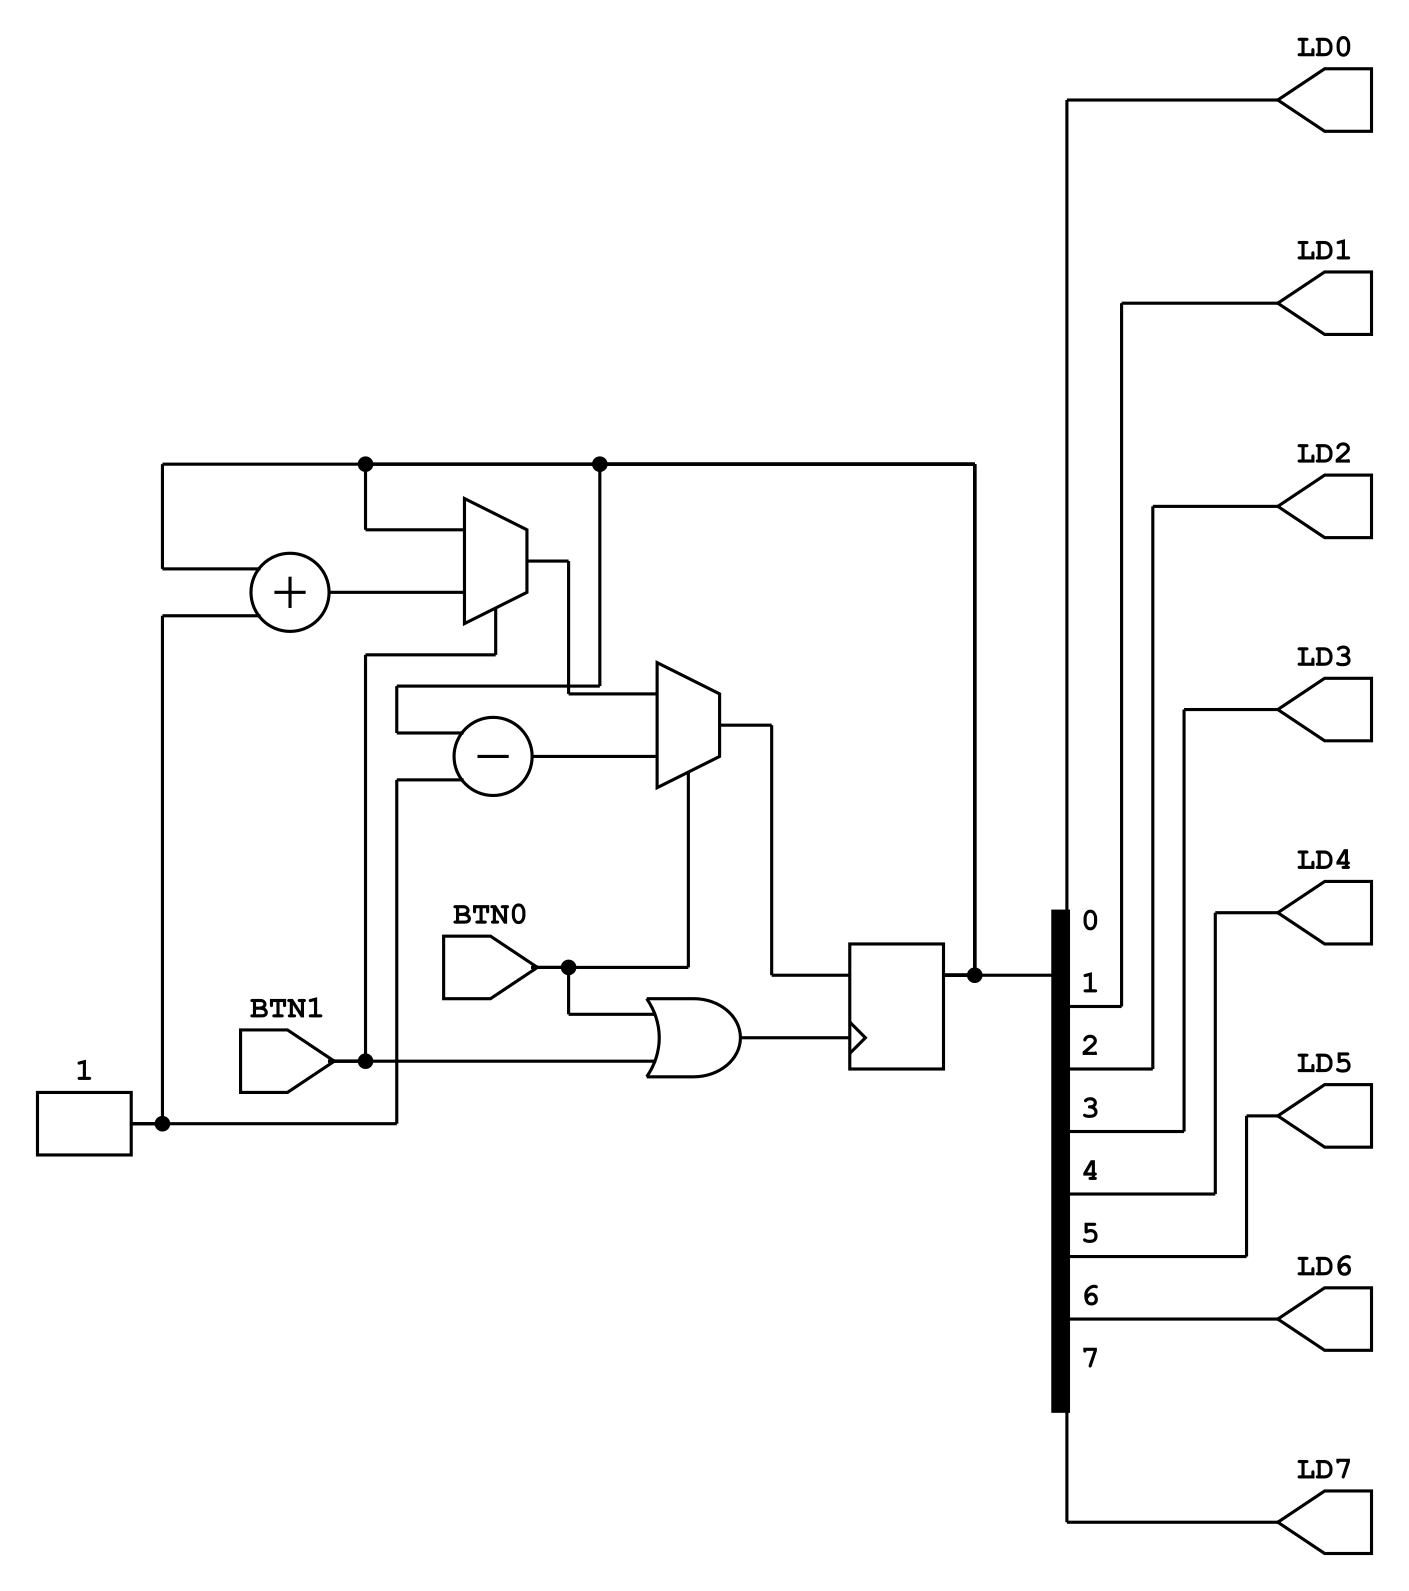
\includegraphics[width=0.5\linewidth]{assets/counter.png}
    \centering
    \caption{Loģisko elementu konfigurācija "pieskaitītājs un atņēmējs"}
    \label{fig:counter}
\end{figure}

Attēlā \ref{fig:counter} redzama shēmtehnika, kas realizē šādu "pieskaitītāja un
atņēmēja" aparatūras loģisko elementu konfigurāciju.

Šī shēmtehnika arī ilustrē visus iepriekšminētos projektēšanas pamatelementus.
Konfigurācijā redzami divi ievadsignāli "BTN0" un "BTN1" un astoņi "LD{0-7}"
izvadsignāli. Papildus konfigurācijā izmantots astoņu bitu atmiņas flip-flop
reģistrs (taisnstūris ar trijstūri), signālu multipleksors, kas atkarībā no
"nosacījuma" signāla ārā izvada vai nu vienu signālu vai otru (trapece),
konstants astoņu bitu signāls ar vieninieka vērtību (taisntūris ar "1"). Kad
"BTN0" signāls top no 0 par 1, reģistrā "1" tiek atņemts vieninieks. Kad "BTN1"
signāls top no 0 par 1, reģistrā "0" tiek pieskaitīts vieninieks. Astoņu bitu
reģistra "1" bitu vērtība tiek izvadīta izvadsignālos "LD{0-7}". Vērts pieminēt,
ka "+" un "-" šajā ilustrācijā ir abstrakcijas, ar kurām patiesībā domāti
elementi 1) astoņu bitu "full adder" un 2) astoņu bitu "full subtractor".

Lai no \gls{hdl} valodas iegūtu attēlā \ref{att:counter} redzamo loģisko
elementu konfigurāciju, ir nepieciešams veikt projektējuma sintēzi, kas pārveido
augsta abstrakcijas līmeņa \gls{hdl} aprakstu uz zema abstrakcijas līmeņa
\gls{netlist} jeb elektrisko savienojumu aprakstu, kuru, savukārt, var realizēt
īstā aparatūrā, kas aprakstīts nodaļā \ref{sec:fpgaboard}.

Šī ilustrācija ir izveidota izmantojot "yosys" atvērtos rīku \gls{hdl} sintēzei
un "netlistsvg" atvērto rīku sintezētā elektronikas apraksta ilustrācijai. Šīs
digitālās aparatūras Verilog projekta avota kods un ilustrācijas kods ir
pieejams šī projekta avota koda repozitorijā. \cite{VeinbahsKrisjanisTestbed}
Papildus tas ir pieejams arī pielikumā \ref{att:counter}.

\section{FPGA attīstītājrīki}
\label{sec:fpgaboard}

Lai digitalizētu digitālas aparatūras prototipēšanas fāzi, darbā izstrādātā
platforma abstrahē attālinātu mijiedarbību ar \glslink{board}{digitālu iekārtu
projektēšanas aparatūru} jeb, precīzāk, mijiedarbību ar \glslink{board}{FPGA
attīstītājrīku aparatūru}.

Iepriekšējā nodaļā ir aprakstīta digitālās aparatūras projektēšana, taču, lai
saprastu kā strādā izstrādātā digitālās aparatūras attālinātās prototipēšanas
platforma, ir noderīgi apskatīt kā \glslink{board}{FPGA attīstītājrīku
aparatūra} iederās aparatūras prototipēšanas fāzē.

Ja uz papīra vai datorā ir izstrādāts digitālās aparatūras projektējums jeb
savienojumi, signāli un loģiskie elementi un ja šis projektējums ir sintezēts
elektrisko savienojumu aprakstā jeb \gls{netlist}, tad ir divas iespējas kā to
realizēt fiziskā, lietojamā digitālā aparatūrā: 1) ražot mikroshēmu kādā
silīcija plates ražotnē \cite{WikiFabs} vai 2) \glslink{board}{FPGA
attīstītājrīku aparatūrā} augšupielādēt aparatūras loģisko elementu
konfigurāciju.

Attēlā \ref{fig:fpgalayers} redzama \gls{fpga} arhitektūra, kas sastāv no diviem
slāņiem - lietotāja un konfigurācijas slāņa, kur lietotāja slānis realizē vēlamo
digitālo aparatūru un konfigurācijas slānis satur atmiņu, kurā iekodēta šīs
aparatūras loģisko elementu konfigurācija, kuru izmanto lietotāja slānis.
\cite[para. II]{HerreraAlzu2013}

Atkarībā no izmantotās \gls{fpga} mikroshēmas, ir atkarīgs, cik apjomīgu
aparatūru ir iespējams projektēt. Programmaparatūras apjomu mēra \gls{lcs} jeb,
cik loģikas elementi ir nepieciešami, lai to realizētu. Piemēram, Digilent Anvyl
Spartan-6 FPGA \cite{XilinxSpartan6}, kas primāri izmantots darba izstrādē, satur 43661 \gls{lcs},
bet, piemēram, Lattice Semiconductor iCEstick ICE40-HX1K FPGA, kas izmantots mazāk un
eksperimentālos nolūkos, satur 1280 \gls{lcs} \cite{iCE40}.

\begin{figure}[H]
    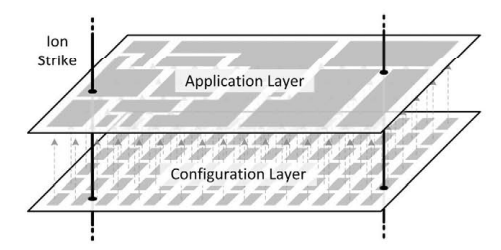
\includegraphics[width=0.5\linewidth]{assets/a-c-layers.png}
    \centering
    \caption{\gls{fpga} loģisko elementu konfigurācijas realizācija.
    \cite[para. II]{HerreraAlzu2013}}
    \label{fig:fpgalayers}
\end{figure}

Tomēr, lai attēlā \ref{fig:fpgalayers} redzamo konfigurācijas slāni
noprogrammētu ar vēlamo aparatūras loģisko elementu konfigurāciju, ir
nepieciešama papildus elektronika, kas ierakstīs vēlamo informāciju šajā
konfigurācijas slāņa atmiņā.

\glslink{board}{FPGA attīstītājrīku aparatūra} ir digitāla aparatūra, kas
abstrahē darbu ar \gls{fpga} mikroshēmu. Piemērs šādai
\glslink{board}{aparatūrai}, kas arī tika izmantota darbā aprakstītās platformas
izstrādei, ir Digilent Anvyl attīstītājrīks, kas redzams attēlā
\ref{fig:anvylexplained} un kas satur Xilinx Spartan-6 \gls{fpga} mikroshēmu, kā
arī \glslink{uart}{USB-UART} savienojumu, lai nodrošinātu attīstītājrīka
pārvaldību no datora, kas arī ir galvenais izmantotais mijiedarbības mehānisms
ar attīstītājrīku izstrādātajā platformā.

\begin{figure}[H]
    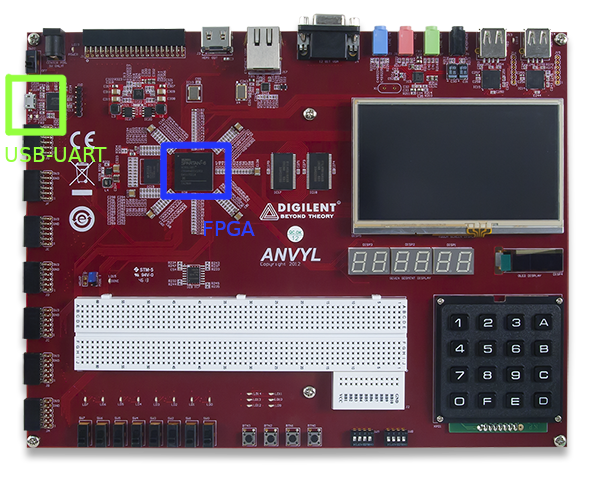
\includegraphics[width=0.7\linewidth]{assets/anvyl-explained.png}
    \centering
    \caption{Digilent Anvyl attīstītājrīks (viss attēls), Xilinx Spartan-6
        \gls{fpga} (zilais taisnstūris ar "\gls{fpga}") un \glslink{uart}{USB-UART} savienojums
        (zaļais taisnstūris ar \glslink{uart}{"USB-UART"}).}
    \label{fig:anvylexplained}
\end{figure}

\section{Aktieru modelis}
\label{sec:actormodel}

Lai modelētu platformā fiziski pieejamo digitālo aparatūru un platformas
lietotājus, tiek izmantots \glslink{actor}{aktieru} modelis.
\glslink{actor}{Aktieru} modelis apraksta veidu kā realizēt vienotu
atteikumnoturīgu informācijas sistēmu, kas sastāv no vairākām atsevišķām,
paralēli darbinātām mazākām informācijas sistēmām - \glslink{actor}{aktieriem}.
\glslink{actor}{Aktieru} modelī \glslink{actor}{aktieri} var 1) sūtīt ziņas, 2)
izveidot jaunus \glslink{actor}{aktierus} un 3) definēt kā reaģēt uz ziņām kas
tiek adresētas tiem pašiem. \cite[p. 1]{CarlHewitt2010}

Lai modelētu fizisku attīstītājrīku \glslink{board}{aparatūras} un lietotāju
savienojumus, ir noderīgs \glslink{actor}{aktieru} modelis, kura pamatprincips
ir, ka \glslink{actor}{aktieriem} piemīt laicīgs dzīvescikls tātad jebkurā brīdī
tie var sākt darboties vai beigt darboties, jo gan \glslink{board}{aparatūrai},
gan lietotājiem var pazust interneta savienojums.
\cite[p. 6]{CarlHewitt2010} 
 
Šī īpatnība ir noderīga darba ietvaros, jo fiziskā \glslink{board}{aparatūra}
var salūzt, zaudēt elektrību, zaudēt interneta savienojumu, utml. Savukārt,
lietotāji platformai var pieslēgties un no tās atvienoties. Kā arī šis modelis
ir vērtīgs, jo eksistē publiski pieejami satvari, kas ir izstrādāti pēc šī
modeļa un tātad ļauj projektēt šāda veida sistēmas. Šī darba ietvaros ir
izmantots satvars Akka, programmēšanas valodā Scala. Akka satvars ir pieejams
Java, Scala un .NET programmēšanas valodās, kā arī konceptuāli līdzīgi satvari
eksistē arī daudzās citās valodās, piem. Erlang valodā OTP satvars, Rust valodā
Actix, Haskell valodā Cloud Haskell, utml, taču Scala valoda ir izvēlēta, jo tā
ļauj programmētājam vieglāk rakstīt funkcionālu kodu, izcelt funkcijas, kam
piemīt blakusefekti, tādējādi atvieglojot platformas koda uzturamību un
lietojamību. 

\begin{figure}[H]
    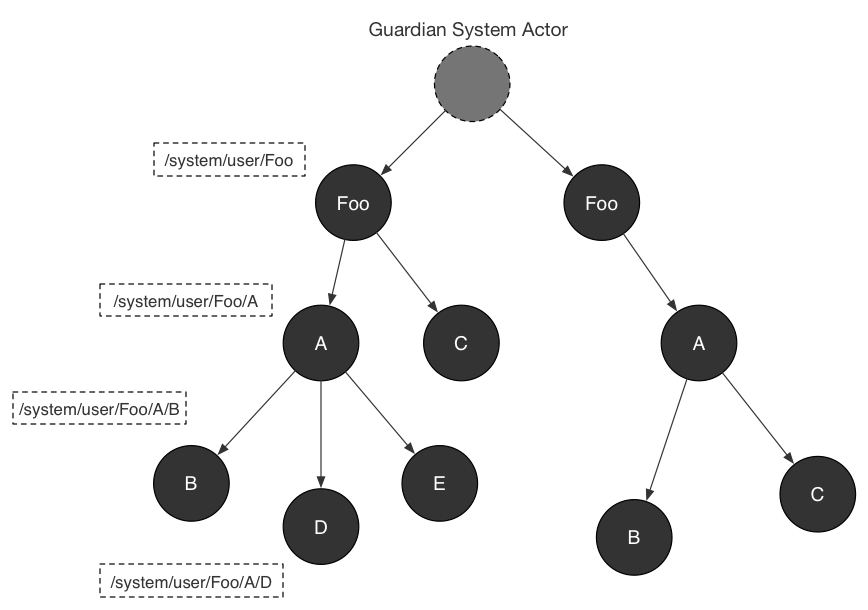
\includegraphics[width=0.5\linewidth]{assets/akka-actor-hierarchy-gray.png}
    \centering
    \caption{\glslink{actorsystem}{Aktieru modeļa sistēmas} hierarhija.
    \cite[sl. 34]{MarkusJuraAkka}}
    \label{fig:actorsystem}
\end{figure}

Attēlā \ref{fig:actorsystem} redzama \glslink{actor}{aktieru} modelim specifiskā
\glslink{actorsystem}{aktieru sistēmas} hierarhija - kuru "bērna"
\glslink{actor}{aktieri} izveidojis kurš "vecāka" \glslink{actor}{aktieris}.
\glslink{actorsystem}{aktieru sistēmas} parasti sastāv no sistēmas
\glslink{actor}{aktieriem} un lietotāja \glslink{actor}{aktieriem}, parasti ir
viens saknes aizbildnības \glslink{actor}{aktieris}, kas izveido sistēmas un
lietotāju aizbildnības \glslink{actor}{aktierus}, savukārt, programmētājs
izmanto šo lietotāju aizbildnības \glslink{actor}{aktieri}, lai izveidotu savu
biznesa loģikas saknes \glslink{actor}{aktieri}, kas savukārt izveidos veselu
biznesa loģikas \glslink{actor}{aktieru} hierarhiju atbilstoši vajadzībām.
\cite[para. The Akka actor hierarchy]{LightbendAkka2619}

\section{Notikumu sistēmas}
\label{sec:eventsourcing}

Lai realizētu viegli testējamus \glslink{actor}{aktieru} modeļus lietotāju un
aparatūras mijiedarbībām ar platformu, platformā ir izmantotas notikumu
sistēmas, kas nošķir saņemtās, izsūtītās ziņas, aktuālo sistēmas stāvokli un
izpildītos blakusefektus. Notikumu sistēma ir tāda informācijas sistēma, kas
apstrādā komandas jeb vēlamās izmaiņas sistēmā, potenciāli akceptē komandas
notikumos jeb veiktajās izmaiņās, izmaina sistēmas stāvokli atbilstoši šiem
notikumiem jeb izmaiņām kā arī izpilda blakusefektus jeb reakcijas atbilstoši
šiem notikumiem, lai izmainītu kādas ārējas sistēmas stāvokli.
\cite[para. 3.2.3]{JohnsenEspen2018}

Notikumu sistēmas pamatā ir notikumu dzinējs, kas realizē vēlamo sistēmas
loģiku. Šāds dzinējs, to mazliet abstrahējot, sastāv no trīs detaļām: 1)
stāvoklis jeb dati, kas tiek sākotnēji izveidoti un tad mainīti atbilstoši
notikumiem, 2) funkcija, kas lasa šobrīdējo stāvokli un validē komandas jeb
noraida tās vai akceptē tās notikumos un 3) funkcija, kas reaģē uz notikumiem
jeb attīsta aktuālo stāvokli jeb datus un izpilda notikumu blakusefektus. Attēlā
\ref{fig:eventengine} redzams šādas sistēmas dzīvescikls jeb stāvoklis,
validācijas un attīstības funkcijas un izpildītie blakusefekti.

Notikumu sistēmas iet roku rokā ar iepriekšminēto \glslink{actor}{aktieru}
modeli. Katru \glslink{actor}{aktieri} var realizēt kā notikumu sistēmu - 1)
\glslink{actor}{aktieris} saņem ziņas no citiem \glslink{actor}{aktieriem} jeb
komandas jeb vēlamās izmaiņas, tās tiek validētas jeb akceptētas vai noraidītas,
2) komandas rezultē akceptētos notikumos, 3) notikumi izmaina aktuālo stāvokli
un rezultē blakusefektos. 

\begin{figure}[H]
    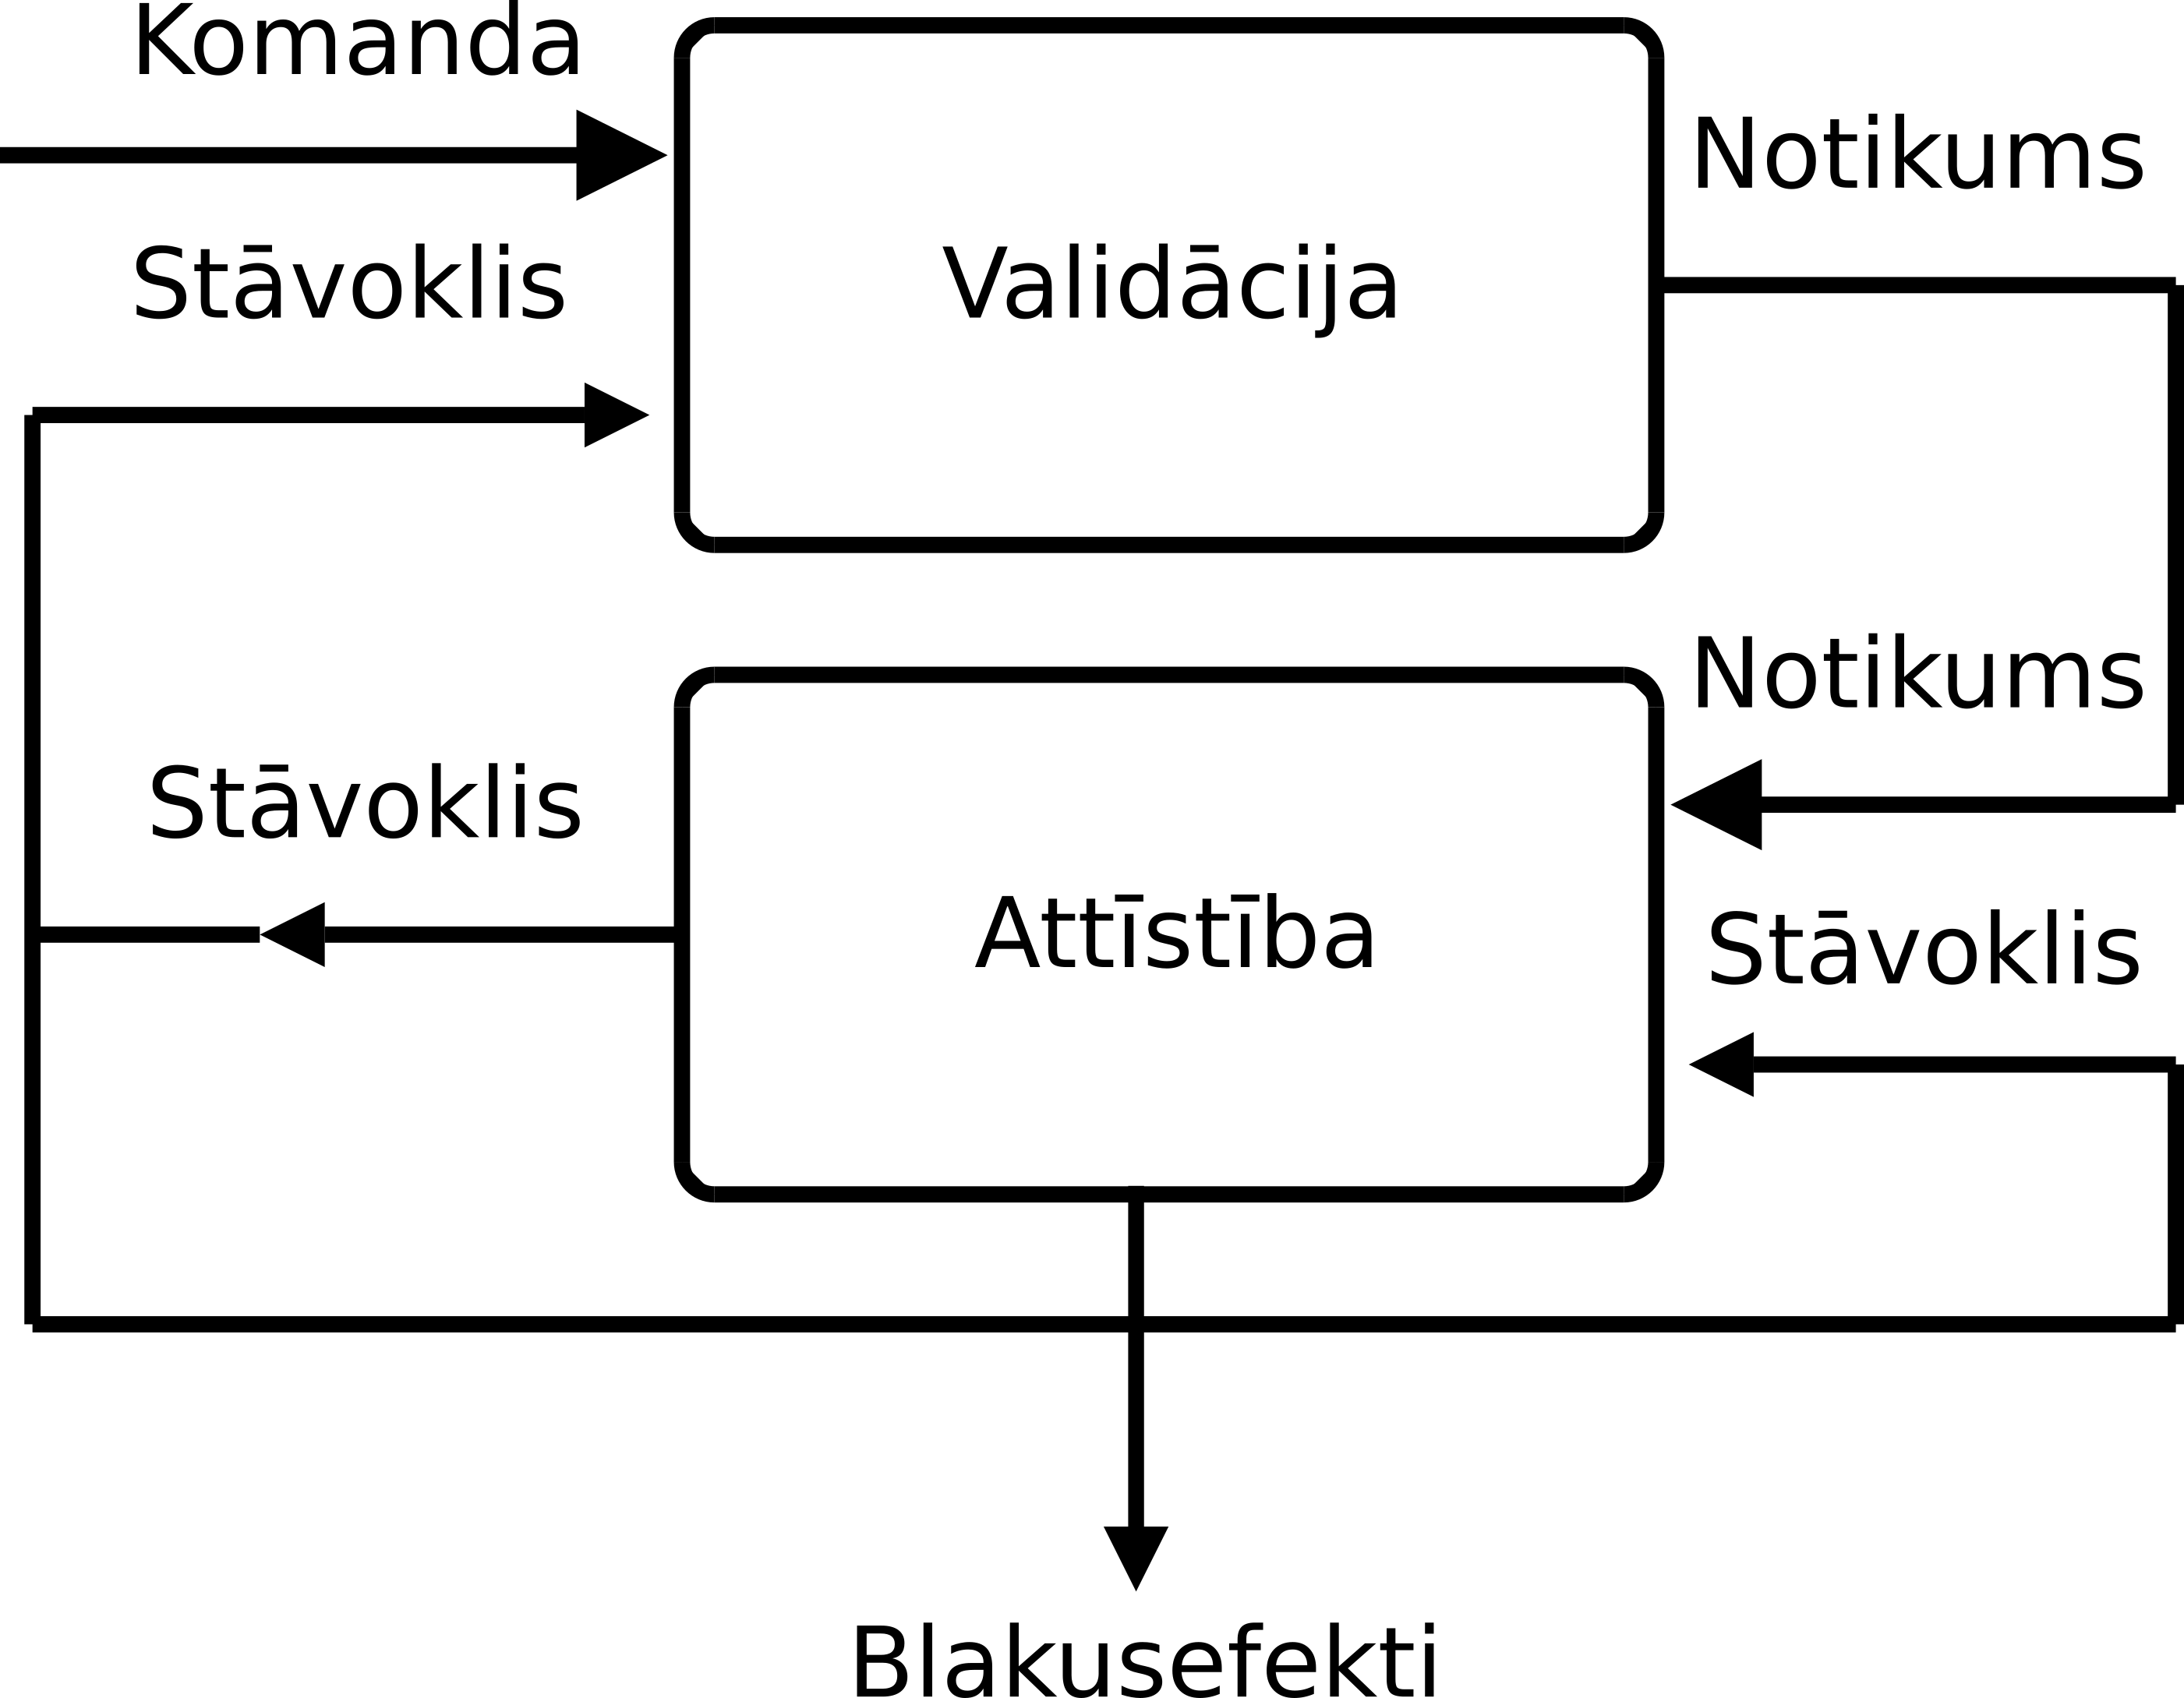
\includegraphics[width=0.5\linewidth]{assets/event-sourcing-decider.png}
    \centering
    \caption{Notikumu sistēmas apstrādes cikls. Papildināts no tiešsaistes avota. \cite{JeremieChassaing2021}}
    \label{fig:eventengine}
\end{figure}

Darba ietvaros katram attīstītājrīkam tiek piesaistīta viena vai vairākas
pārvaldības notikumu sistēmas jeb "aģenti". Aģents ir paredzēts, lai pārvaldītu
video straumēšanu, \glslink{firmware}{programmaparatūras} augšupielādi, seriālā
porta monitorēšanu, un viss tiek realizēts izmantojot komandas, notikumus un
blakusefektus. Tai skaitā arī platformas lietotāji attālināti mijiedarbojoties
ar attīstītājrīkiem izmanto virtuālās \glslink{vinterface}{saskarnes}, piem.
MinOS., kas arī ir realizētas kā notikumu sistēmas. Pašā platformā,
centralizētajā \glslink{server}{serverī}, lietotāju un aģentu apkalpošanas
mehānismi ir realizēti izmantojot notikumu sistēmas un \glslink{actor}{aktieru}
modeli. 

\section{Seriālā komunikācija}
\label{sec:serial}

Pieņemot, ka ir iespējama centralizēta platforma, kas aprakstīta vēlākās
nodaļās, kas nodrošina datu apmaiņu starp lietotājiem un
\glslink{board}{aparatūru}, ir jāņem vērā, ka, projektējot elektroniku, tomēr ir
ļoti skaidri jādefinē, ko īsti nozīmē datu apmaiņa ar
\glslink{board}{aparatūru}.

Šī darba ietvaros datu apmaiņa ar attīstājrīku \glslink{board}{aparatūru} ir
realizēta izmantojot \glslink{serialport}{seriālo komunikāciju}. Precīzāk,
\gls{fpga} tiek augšupielādēta \gls{firmware}, lai seriāli komunicētu ar
attīstītājrīkā esošu \gls{uart} kontrolieri ar diviem "RX" un "TX" signāliem,
savukārt, \gls{uart} kontrolieris šo visu pārraida pāri \gls{usb} savienojumam
\cite[para. USB-UART Bridge]{DigilentAnvylReference}, un šos datus saņem
attīstītājrīkam ar \gls{usb} vadu pievienots mikrokontrolieris, kas satur
platformas programmatūru, ko savukārt sauc par "\glslink{agent}{aģentu}". Šo
mehānismu ar \gls{ttl}, \gls{usb}, \gls{uart} komunikāciju var apskatīt attēlā
\ref{fig:agentcomms}.


\begin{figure}[H]
    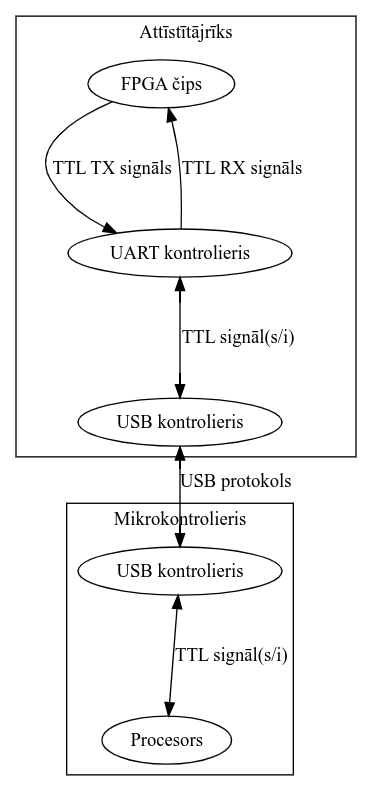
\includegraphics[width=0.3\linewidth]{assets/agentcomms-grey.png}
    \centering
    \caption{Datu apmaiņa starp attīstītājrīku un platformas "\glslink{agent}{aģentu}"}
    \label{fig:agentcomms}
\end{figure}

Ņemot vērā, šo attīstītājrīkā pieņemto komunikācijas modeli, vienīgais, ko
atliek realizēt pašam, ir projektēt \gls{ttl} seriālo komunikāciju, izmantojot
\gls{uart} mehānismu, lai nodrošinātu baitu apmaiņu starp ierīcēm. Attēlā
\ref{fig:serialframe} redzams seriālās komunikācijas kadrs iekodēts spriegumā,
ko attiecīgi var jau noprojektēt Verilog valodā, tādējādi nodrošinot
\glslink{fullduplex}{pilndupleksa} \gls{uart} baitu datu apmaiņu starp ierīcēm.
Šī darba ietvaros tika izmantota seriālā komunikācija "8-N-1" jeb ar 8 datu
bitiem, bez paritātes bita un ar vienu "stop" bitu.

\begin{figure}[H]
    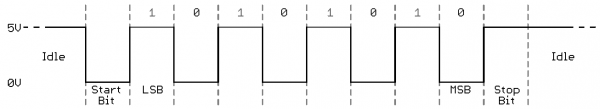
\includegraphics[width=0.7\linewidth]{assets/ttl-serial-gray.png}
    \centering
    \caption{Seriālās komunikācijas kadrs iekodēts fiziskā signālā}
    \label{fig:serialframe}
\end{figure}
